\section{Correlations in the 2D Ising Model}

We discussed the cluster algorithm for the 2d Ising model in class. We saw that the
partition function could be written as
%
\begin{equation}
    Z = \sum_{\{\sigma\}} \prod_{\langle i j \rangle} \sum_{n_{ij}=0}^1
    \bigl((1 - p) \delta_{n_{ij},0} + p \delta_{\sigma_i,\sigma_j} \delta_{n_{ij},1}\bigr),
\end{equation}
%
in the Swendsen--Wang algorithm,
where \(\langle i j \rangle\) refers to all nearest neighbour pairs of atoms.
In this problem, you should start from this code and add measurements to measure the
correlation length near the critical value of \(J\), or \(P=1 - \exp(-2J)\).

As the Ising model approaches its critical point, the size of spatial clusters grows. It is
this growth in the average size of clusters responsible for diverging correlation
length at \(T_c\) and the corresponding second-order phase transition. The cluster algorithm
avoids the critical slowing down that comes from the slow evolution through phase space of
the simple, local site Metropolis algorithm.

In this problem, you should measure the spatial correlation between spins. The simplest
correlator is
%
\begin{equation}
    \expval{ \sigma(x_1, y_1) \sigma(x_2, y_2) }.
\end{equation}
%
But the statistical errors are much smaller if on each configuration of an \(N \times N\)
lattice you calculate
%
\begin{equation}
    \Sigma_x(x) = \frac{ 1 }{ N } \sum_y \sigma(x, y),
\end{equation}
%
and
%
\begin{equation}
    \Sigma_y(y) = \frac{ 1 }{ N } \sum_x \sigma(x, y),
\end{equation}
%
and then calculate
%
\begin{equation}\label{eq:Sigmaz}
    \Sigma(z) = \frac{ 1 }{ 2N } \biggl( \sum_x \Sigma_x(x) \Sigma_x(x+z)
    + \sum_y \Sigma_y(y) \Sigma_y(y+z) \biggr).
\end{equation}
%
On a periodic lattice, the ensemble average \(\expval{\Sigma(z)}\) is only a
function of \(\abs{z}\). Above \(T_c\),
where there is no spontaneous magnetization, \(\expval{\Sigma(z)}\) has the form
%
\begin{equation}\label{eq:Sigmazbar}
    \expval{\Sigma(z)} = a \bigl(\exp(-z / b) + \exp(-(N - z) / b)\bigr).
\end{equation}

First, we need to write the cluster algorithm for the Ising model.
Consider a 2D lattice of atoms in the presence of a \(z\)-directed magnetic field of strength
\(B\). Suppose that all atoms are identical spin-\(1/2\) systems.
We define the lattice in Snippet~\ref{lst:lattice},
where it is a \code{Matrix} containing spins of values \(s_i = 1\) (spin up) or
\(s_i = -1\) (spin down), where \(s_i\) is (twice) the \(z\)-component of the \(i\)th
atomic spin. The total energy of the system is written as:
%
\begin{equation}
    E = -J \sum_{\langle i j \rangle} s_i s_j - B \sum_{i} s_i,
\end{equation}
%
where \(J\) is the exchange energy.

%
\begin{algorithm}
    \caption{Define the 2D lattice for the Ising model.}
    \label{lst:lattice}
    \begin{juliacode}
        struct Lattice{T} <: AbstractMatrix{T}
            spins::Matrix{T}
        end
    \end{juliacode}
\end{algorithm}
%
And for different simulation algorithms, we define several types, as in
Snippet~\ref{lst:alg}, where \code{Basic} is the simplest algorithm
denoting flipping spins one by one, and \code{SwendsenWang} is the cluster
algorithm we will discuss below.

\begin{algorithm}
    \caption{Different simulation algorithms.}
    \label{lst:alg}
    \begin{juliacode}
        abstract type Algorithm end
        struct Basic <: Algorithm end
        struct Checkerboard <: Algorithm end
        struct SwendsenWang <: Algorithm end
    \end{juliacode}
\end{algorithm}

The \code{Basic} algorithm, as in Snippet~\ref{lst:basic},
is the slowest one when doing the simulation. However, it is easy to implement
and less error-prone.

\begin{algorithm}
    \caption{The simplest algorithm: flipping spins one by one.}
    \label{lst:basic}
    \begin{juliacode}
        function simulate!(lattice::Lattice, β, J, B, ::Basic)
            for index in eachindex(lattice)
                trial_spin = flipspin!(lattice, index)  # Trial move
                eᵢ_old = energy(lattice, index, J, B)
                eᵢ_new = energy(sum(neighborspins(lattice, index)), trial_spin, J, B)
                P = exp(-β * (eᵢ_new - eᵢ_old))
                if P > rand()
                    lattice[index] = trial_spin  # Accept the trial move
                end
            end
            return lattice
        end
    \end{juliacode}
\end{algorithm}

The Metropolis--Hastings approach to the Ising model, which completely avoids the use of the mean
field approximation, is based on the following algorithm, i.e.,
step through each atom in the array in turn:
%
\begin{itemize}
    \item For a given atom, evaluate the change in energy of the system, \(\Delta E\), when
          the atomic spin is flipped.
    \item If \(\Delta E < 0\) (lowering energy), then flip the spin.
    \item If \(\Delta E > 0\) then flip the spin with probability
          \(P=\exp(-\beta \Delta E)\).
\end{itemize}
%
Repeat the process many times until thermal equilibrium is achieved.

\begin{figure}[hbt]
    \centering
    \begin{subfigure}{0.49\textwidth}
        \centering
        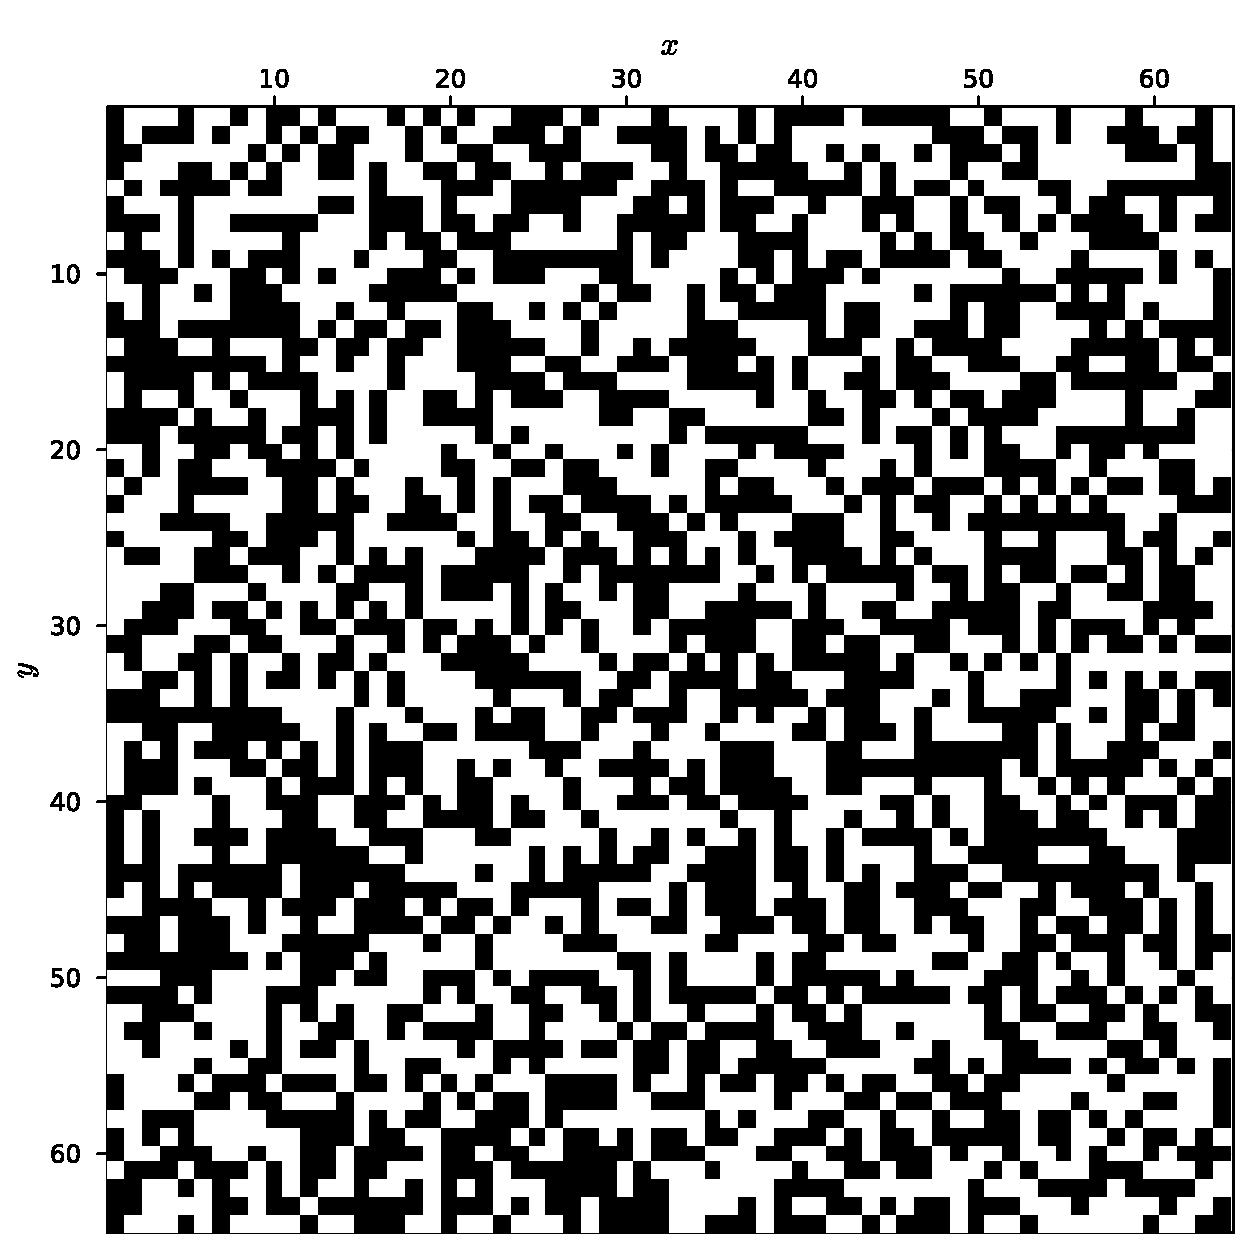
\includegraphics[width=\linewidth]{basic_J=0.455_t=0}
    \end{subfigure}
    \hfill
    \begin{subfigure}{0.49\textwidth}
        \centering
        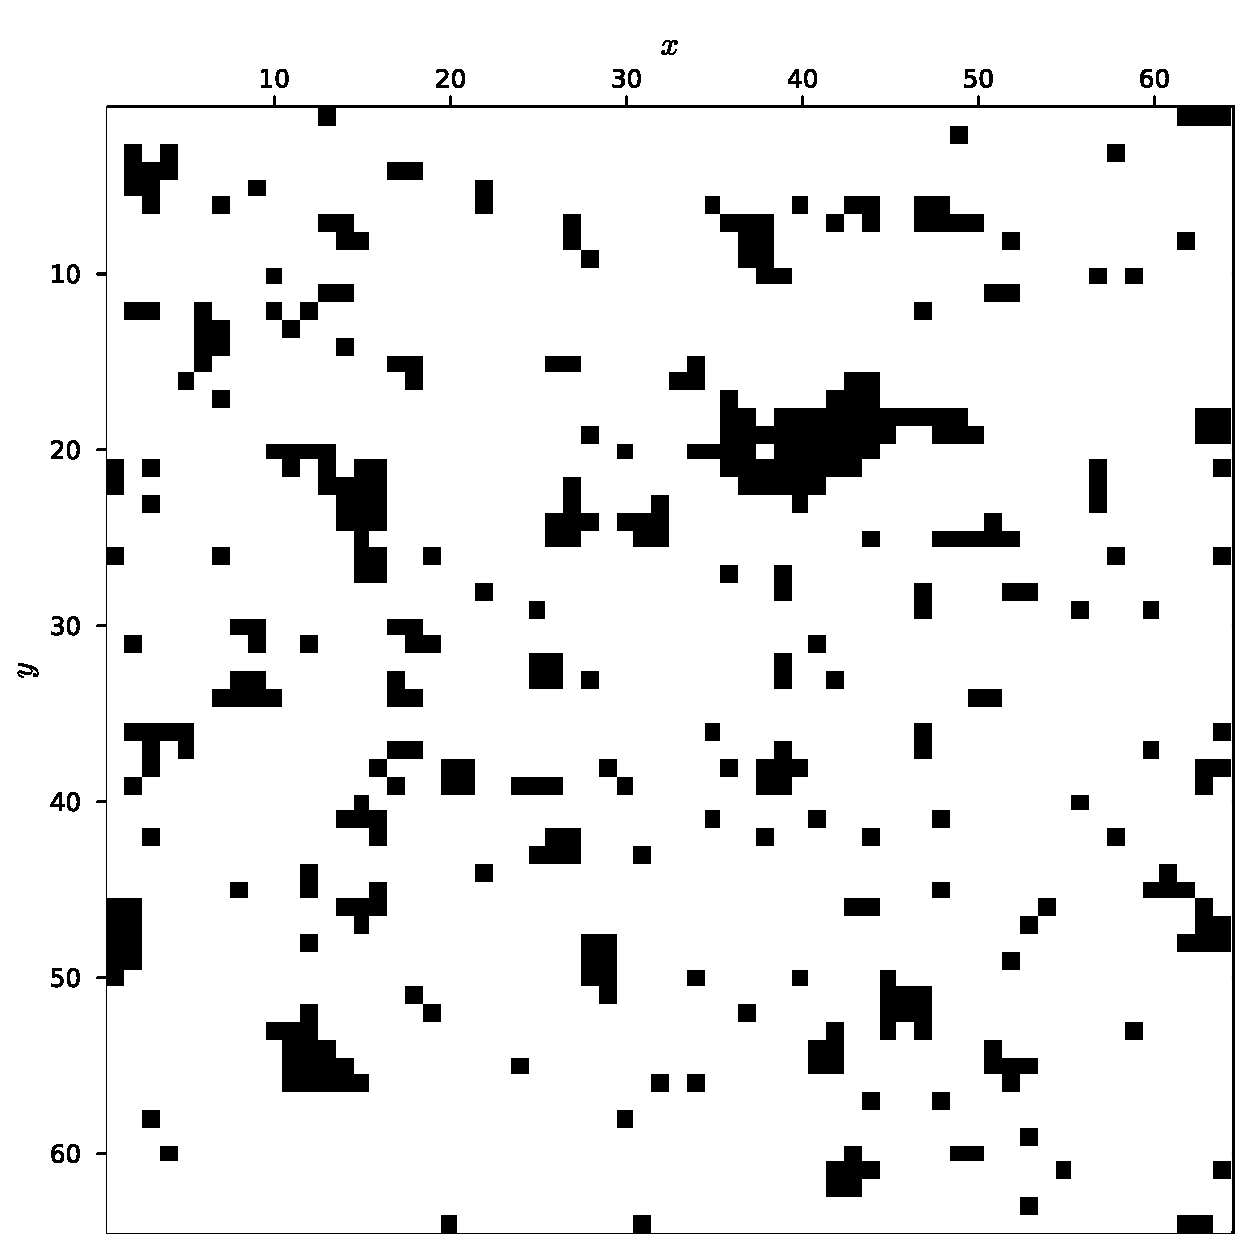
\includegraphics[width=\linewidth]{basic_J=0.455_t=5000}
    \end{subfigure}
    \caption{Magnetization pattern of a \(64 \times 64\) array of ferromagnetic atoms in
        thermal equilibrium and in the absence of an external magnetic field at \(t = 0\)
        (left), and \(t = 5000\) (right), with \(J = 0.455\). Black/white squares indicate
        spin up and spin down, respectively. The simulation is done using the \code{Basic}
        algorithm.}
    \label{fig:rand_J=0.455}
\end{figure}

In Snippet~\ref{lst:basic}, we use function \code{neighborspins} to find all the neighboring
spins \(s_j\) of a specific spin \(s_i\). Notice we do not update the spin immediately
since it is just a trial move at the beginning. We only update it until the probability of
the flipping is larger than a (uniformly distributed between \(0\) and \(1\)) random number.
Since for any fixed \(P\), the probability of generating a random number that is smaller
than \(P\) is \(P\). Therefore, we accept the trial move with probability \(P\).
We plot the results of one simple simulation in Figure~\ref{fig:rand_J=0.455},
with the initial spins randomly choosen.

\begin{algorithm}
    \caption{The Swendsen--Wang algorithm for simulating the Ising model.}
    \label{lst:cluster}
    \begin{juliacode}
        function simulate!(lattice::Lattice, β, J, B, ::SwendsenWang)
            index = rand(CartesianIndices(lattice))
            P = 1 - exp(-β * (2J + B))
            recursive_flipspin!(lattice, index, lattice[index], P)
            return lattice
        end
    \end{juliacode}
\end{algorithm}

For the cluster algorithm, we need to adopt an recursive scheme, as shown in
Snippet~\ref{lst:cluster}. The recursive spin-flipping method is defined in
Snippet~\ref{lst:recur}.

In each timestep, we randomly select one atom, flip its spin, and for each of its four
neighbors, see if it has a ``link'' connecting the spins (i.e., the ``bond'' is \emph{open}).
If so, flip that spin with probability \(P = 1 - \exp(-2J)\).
Recursively repeat these steps until we have reached the end of the tree where
every ``bond'' is closed.

\begin{algorithm}
    \caption{The recursive spin-flipping method.}
    \label{lst:recur}
    \begin{juliacode}
        function recursive_flipspin!(lattice::Lattice, index, spin₀, P)
            spin = flipspin!(lattice, index)
            for index′ in findneighbors(lattice, index)
                if lattice[index′] == spin₀ && P > rand()
                    recursive_flipspin!(lattice, index′, spin₀, P)
                end
            end
            return spin
        end
    \end{juliacode}
\end{algorithm}

\subsection{Measuring this observable}

Measure the correlation in \(\eqref{eq:Sigmaz}\). Even
though the cluster algorithm produces decorrelated configurations quite rapidly, you should
still do some number of spin-flip updates between each measurement. Ten updates is a
reasonable choice.

When you measure \(\eqref{eq:Sigmaz}\) on a configuration, you will end up with \(N\)
values, one for each value of \(z\). For each value of \(z\), you can also determine the
error on the average value using the statistical methods of Problem Set 3.

\Question{} Measure \(\eqref{eq:Sigmaz}\) on systems with values for \(J\) of \(0.435\),
\(0.430\), \(0.425\). (Note that the critical value is \(J_c = 0.4406868\) and higher
temperatures correspond to lower values of \(J\), since we wrote \(J = \bar{J} / k_B T\).

\subsection{Determining the correlation length}

In \(\eqref{eq:Sigmazbar}\), \(b\) is the correlation length, which should grow as
\(J \rightarrow J_c\).

\Question{} You can fit your data to the form of \(\eqref{eq:Sigmazbar}\) to find \(b\)
using the curve fit function \code{curve_fit} from
\href{https://github.com/JuliaNLSolvers/LsqFit.jl}{\code{LsqFit.jl}}.

You should include the statistical error on each correlator point in your inputs to
\code{curve_fit}.
You don't need to calculate the error on the returned value of the correlation length,
\(b\), but this can be done with jackknife methods.


\Question{} Report on your determination of \(b\) for each of the \(J\) values you
simulated. Do you find the expected change in \(b\) as \(J \rightarrow J_c\)?
